\documentclass[11pt,a4paper]{article}
\usepackage{fontspec}
\setmainfont{Times New Roman}
\setmonofont{Consolas}[Scale=0.9]
\usepackage[latvian]{babel}
\usepackage[margin=2.2cm]{geometry}
\usepackage{amsmath}
\usepackage{graphicx}
\usepackage{booktabs}
\usepackage{hyperref}
\usepackage{enumitem}
\setlist{nosep}
\setlength{\parskip}{4pt}
\setlength{\parindent}{0pt}

\title{\vspace{-1.5cm}Mazais praktiskais darbs: X-Sudoku ar Simulated Annealing}
\author{Kristiāns Rasiņš \\ kr26040}
\date{2026. gada oktobris}

\begin{document}
\maketitle
\vspace{-0.8cm}

\section{Uzdevuma formulējums}

Izvēlējos X-Sudoku. Tas ir parasts Sudoku, tikai ar vienu papildu noteikumu: abās galvenajās
diagonālēs arī katram ciparam jāparādās tieši vienu reizi. Vispārīgi laukums ir $n\times n$, kur
$n=b^2$ ($b=2,3,4,5$, t.i. $4\times4$, $9\times9$, $16\times16$, $25\times25$), un ir doti daži
cipari (``clues''), kurus mainīt nedrīkst. Jāaizpilda pārējās šūnas tā, lai katrā rindā, kolonnā,
$b\times b$ blokā un abās diagonālēs būtu visi cipari $1..n$.

Sudoku īstenībā ir apmierināmības uzdevums, nevis optimizācijas, bet to var pārvērst par
optimizāciju: skaitām, cik noteikumi ir pārkāpti, un to minimizējam. Optimums ir 0 (atrisināts
Sudoku), tāpēc šajā gadījumā ``labākais zināmais risinājums'' visām instancēm ir zināms jau iepriekš,
kas testēšanu padara diezgan ērtu.

\section{Algoritma apraksts}

Viss ir uzrakstīts Python valodā (3.13), tikai ar standarta bibliotēku, bez gataviem optimizācijas
rīkiem. Kods ir mapē \texttt{xsudoku/}.

\subsection*{a) Domēns}

Risinājums ir viss režģis. Plānošanas mainīgie ir tukšās šūnas, vērtību kopa ir $\{1..n\}$, dotās
šūnas ir fiksētas. Sākuma risinājumu taisu tā: katrā blokā ieliek trūkstošos ciparus nejaušā secībā.
Tādējādi bloku noteikums ir izpildīts jau no paša sākuma, un, tā kā gājiens (sk. c) arī maina tikai
šūnas viena bloka iekšienē, tas paliek izpildīts visu laiku. Tas būtībā samazina meklēšanas telpu un
vienu noteikumu no izmaksu funkcijas var izmest.

\subsection*{b) Novērtēšana}

Izmaksas ir dublikātu skaits rindās, kolonnās un abās diagonālēs:
\[
f = \sum_{u \in \text{rindas, kolonnas, 2 diagonāles}} \big(n - |\{\text{dažādi cipari } u\}|\big)
  = \sum_{u}\sum_{v=1}^{n} \max(0,\ \text{cnt}_u(v) - 1).
\]
Visi noteikumi ir ``hard'' un vienādi svarīgi, tāpēc atsevišķus svarus neliku. Bloki netiek skaitīti,
jo tie vienmēr ir korekti. $f=0$ tad un tikai tad, ja režģis ir pareizs X-Sudoku. Katram galarezultātam
vēl atsevišķi pārbaudu visas $3n+2$ vienības ar neatkarīgu funkciju (\texttt{is\_valid\_solution}),
lai būtu drošs, ka nav kļūda inkrementālajā skaitīšanā.

Izmaksas netiek pārrēķinātas no nulles. Glabāju skaitītājus $\text{cnt}_u(v)$ katrai vienībai, un pēc
gājiena izmaiņu ($\Delta f$) var izrēķināt $O(1)$ laikā, jo katra šūna pieder ne vairāk kā 4 vienībām.
Bez tā Python versija būtu krietni lēnāka.

\subsection*{c) Gājiens}

Gājiens ir divu brīvo šūnu vērtību apmaiņa (swap) viena bloka ietvaros. Uztaisīju divus variantus:
\begin{itemize}
  \item \textbf{random} -- izvēlas nejaušu bloku (kurā ir vismaz 2 brīvas šūnas) un tajā divas nejaušas brīvas šūnas;
  \item \textbf{conflict} -- pirmo šūnu mēģina izvēlēties tādu, kas pašlaik ir konfliktā (tās cipars
        atkārtojas rindā, kolonnā vai diagonālē; līdz 20 mēģinājumiem), otro ņem nejauši no tā paša bloka.
\end{itemize}
Sākumā bija tikai \textit{random}, bet uz lielākiem laukumiem tas strādāja diezgan slikti, jo lielākā daļa
gājienu aiztiek šūnas, kurās jau viss ir kārtībā. \textit{conflict} variants ir mazliet ``mantkārīgāks'',
bet joprojām ir stohastisks.

\subsection*{d) Algoritms}

Simulated Annealing, praktiski tieši pēc lekcijas pseidokoda \texttt{SIMULATED\_ANNEALING($\varphi, f, V, t, L$)}:
gājienu ar $\Delta f \le 0$ pieņem vienmēr, sliktāku pieņem ar varbūtību $e^{-\Delta f / t[k]}$, un
paralēli atceras labāko redzēto risinājumu. Parametri:
\begin{itemize}
  \item sākuma temperatūra $t_0$ -- standartnovirze $\Delta f$ vērtībām no 200 nejaušiem gājieniem
        sākuma stāvoklī (testos sanāca no 1.2 līdz 2.8);
  \item atdzišana ģeometriska: $t[k] = t_0 \cdot \alpha^k$, $\alpha = 0.999$;
  \item $L[k] = $ brīvo šūnu skaits (konstants visām temperatūrām);
  \item kad $t < 0.01$ (``$t\approx0$''), temperatūru uzsilda atpakaļ uz $t_0$ (reheat) un turpina
        no esošā stāvokļa. To pievienoju pats, jo citādi pēc pirmās atdzišanas viss beidzas, un uz grūtākajām
        instancēm tad parasti vēl paliek daži konflikti;
  \item apstājas, kad $f=0$ vai beidzas laika limits.
\end{itemize}
Parametrus izvēlējos, nedaudz paeksperimentējot ar $16\times16$ instanci (mēģināju $\alpha \in
\{0.99, 0.995, 0.999\}$ un dažādus $L$). Atšķirības nebija pārāk lielas, un pilnīgi drošs, ka šie ir
labākie, neesmu -- visticamāk, ar rūpīgāku pielāgošanu var dabūt vēl kaut ko.

\section{Testēšana}

Testa instances ģenerēju pats (\texttt{generate\_instances.py}): ar parastu pārlases (backtracking)
algoritmu uztaisa pilnu X-Sudoku un tad izņem ciparus, kamēr risinājums joprojām ir viens vienīgs.
Kopā 11 instances no $4\times4$ līdz $25\times25$ ar dažādu doto ciparu daudzumu. Optimālais risinājums
katrai ir zināms (glabājas \texttt{*.solution.txt}), un optimālās izmaksas ir 0.

Katru instanci risināju ar abiem gājienu veidiem, katru 5 reizes ar dažādiem seed. Laika limits vienai
palaišanai: 5\,s ($4\times4$), 20\,s ($9\times9$), 60\,s ($16\times16$), 120\,s ($25\times25$).
Dators: AMD Ryzen 7 5700X, 8 palaišanas paralēli (katra savā procesā), tāpēc laiki ir aptuveni.
Tabulā: \textit{atr.} -- cik no 5 palaišanām atrada optimumu, \textit{laiks} -- vidējais laiks
veiksmīgajās palaišanās sekundēs, \textit{izm.} -- labākās atrastās izmaksas (min/vid/max), ja kāda
palaišana optimumu neatrada.

\begin{center}
\small
\begin{tabular}{lrr|rrr|rrr}
\toprule
 & & & \multicolumn{3}{c|}{random} & \multicolumn{3}{c}{conflict} \\
instance & izmērs & doti & atr. & laiks & izm. & atr. & laiks & izm. \\
\midrule
\csname @@input\endcsname table.tex
\bottomrule
\end{tabular}
\end{center}

\begin{center}
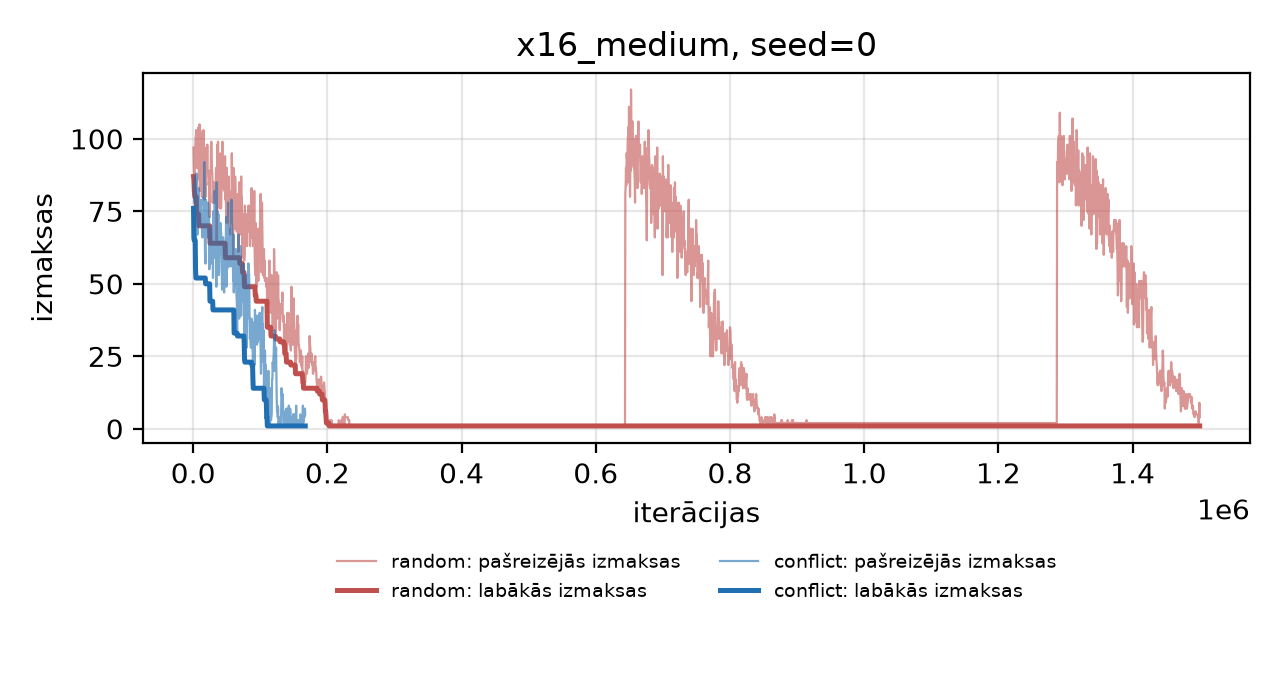
\includegraphics[width=0.8\textwidth]{../results/convergence.png}
\end{center}
\vspace{-0.3cm}
\textit{Izmaksas atkarībā no iterācijām uz x16\_medium. Asie lēcieni uz augšu ir reheat momenti.}

\textbf{Novērojumi.}
\begin{itemize}
  \item Ja doto ciparu ir pietiekami daudz, SA atrod optimumu visās 5 palaišanās un diezgan ātri, pat
        $25\times25$ laukumam ar 58\% dotiem cipariem tas ir ap 2 sekundēm. Kur ir robeža, gan atkarīgs
        no izmēra: $9\times9$ ar 35\% vēl atrisinās bez problēmām, bet $25\times25$ ar 48\% jau
        lielākoties nē.
  \item Uz grūtajām instancēm algoritms ātri nonāk līdz dažiem konfliktiem (x9\_hard un x16\_hard
        izmaksas 1--2), bet pēdējos atrisināt ir grūti, jo tam bieži vajag izjaukt lielu daļu no jau
        ``gandrīz pareizā'' risinājuma. Reheat laikam palīdz (x9\_hard un x25\_hard pa reizei
        atrisinājās), bet ne vienmēr.
  \item \textit{conflict} gājiens gandrīz visur ir labāks: jau uz $9\times9$ tas ir vairākas reizes ātrāks,
        un uz x25\_hard atšķirība ir vislielākā (vidēji 5.6 pret 17.2). Uz $4\times4$ atšķirības nav,
        bet tur jau viss atrisinās uzreiz. Uz x9\_hard abi varianti atrisināja tikai 1 no 5, tā ka
        tur neko īsti secināt nevar.
  \item Godīgi sakot, uz šī uzdevuma SA zaudē parastam backtracking ar MRV heuristiku -- tas
        (tas pats, ko izmantoju instanču ģenerēšanai) jebkuru no šīm instancēm atrisina mazāk nekā
        0.2 sekundēs. Tas laikam nav pārsteidzoši, jo Sudoku ir ļoti ``stingri''
        ierobežots uzdevums, kur constraint propagation strādā ļoti labi, bet lokālajai meklēšanai
        ainava ir diezgan nelīdzena ar daudziem lokāliem minimumiem.
  \item Varbūt varētu uzlabot, ja pirms SA aizpildītu ``acīmredzamās'' šūnas (kurām ir tikai viens
        iespējamais cipars), vai arī ja izmaksu funkcijā kaut kā ņemtu vērā, cik daudz kandidātu katrai
        šūnai paliek. To gan vairs neizmēģināju.
\end{itemize}

\section{Repozitorijs}

Kods, testa instances un rezultāti (\texttt{results/results.csv}):

\url{https://github.com/kristiansrasins/x-sudoku_optimizer}

Palaišana: \texttt{python generate\_instances.py} (instances jau ir repozitorijā),
\texttt{python run\_tests.py}, \texttt{python plot\_convergence.py}.

\end{document}
